\documentclass[12pt]{article}

% ---------------- Packages ----------------
\usepackage[margin=1in]{geometry}
\usepackage{setspace}
\usepackage{graphicx}
\usepackage{amsmath, amssymb}
\usepackage{caption}
\usepackage{float}
\usepackage{hyperref}
\usepackage{booktabs}
\usepackage{enumitem}
\usepackage{indentfirst}

% ---------------- Document Info ----------------
\title{Student Dropout Predictor}
\author{Romerico David}
\date{May 15, 2025}

% ---------------- Begin Document ----------------
\begin{document}

\maketitle

\tableofcontents
\newpage
%---------------------------------------------------

\section{Introduction and Motivation}

For this project, we used the \href{https://archive.ics.uci.edu/dataset/697/predict+students+dropout+and+academic+success}{\textit{Predict Students’ Dropout and Academic Success}} dataset from UC Irvine's Machine Learning Repository. This dataset was constructed by merging several disjoint databases maintained by a higher-education institution, and it contains records from 4,424 undergraduate students enrolled in programs such as agronomy, design, education, nursing, journalism, management, social service, and technology-related disciplines.

Each student is described by 36 features encompassing academic background, demographic attributes, and socio-economic factors available at the time of enrollment. Additionally, it includes academic-performance data collected at the end of the first and second semesters. These features span a range of data types, including real-valued, categorical, and integer values.

The primary objective of this project is to develop a Support Vector Machine (SVM) model to classify students into one of two categories: those who have dropped out and those who have either graduated or are still enrolled. This reduces the original three-class problem into a binary classification task.

Because of the dataset’s potential to effectively predict student dropout and its personal relevance to us as college students, we thought it was worthwhile to explore this set of data that can be used to support early-intervention strategies in educational settings.

%---------------------------------------------------

\section{Data Preprocessing}
\subsection{Plan for Preprocessing}

Given that the dataset contains \textbf{36 features} and \textbf{4,424 instances}, a significant amount of data preprocessing was required to ensure the model could be trained effectively due to the large discrepancy between the number of features and instances. 

Support Vector Machines (SVMs) work by identifying a decision boundary that maximizes the margin between classes. This process relies heavily on dot products and distance calculations, which are sensitive to the magnitudes of individual feature values. If features are on vastly different scales, those with larger numerical ranges can disproportionately influence the model’s decision boundary. So, it is essential to scale all features to a common range.

\textbf{Categorical and nominal features} are particularly difficult to scale consistently, and naïve one-hot encoding can introduce unintended ordinal relationships or other unintended issues. To address these challenges, we applied the following preprocessing steps:

\begin{enumerate}
    \item \textbf{Removed categorical and nominal features} due to the difficulty of scaling them meaningfully and their incompatibility with SVMs (without complex encoding). This step reduced noise and ensured all remaining features were ordinal and numerically meaningful.
    \item \textbf{Assessed the target class distribution} by analyzing the proportion of students who dropped out versus those who did not. An imbalanced class distribution can lead to a skewed model.
    \item \textbf{Statistically analyzed} the remaining features, calculating the minimum, maximum, mean, and median values to identify potential outliers and understand the spread of each variable.
    \item \textbf{Scaled all ordinal features} to ensure they all share a consistent range.
\end{enumerate}

\subsection{Implementation Details and Results}

The following screenshots provide quick snippets of the original raw dataset, which notably contains no missing values.

\begin{figure}[H]
    \centering
    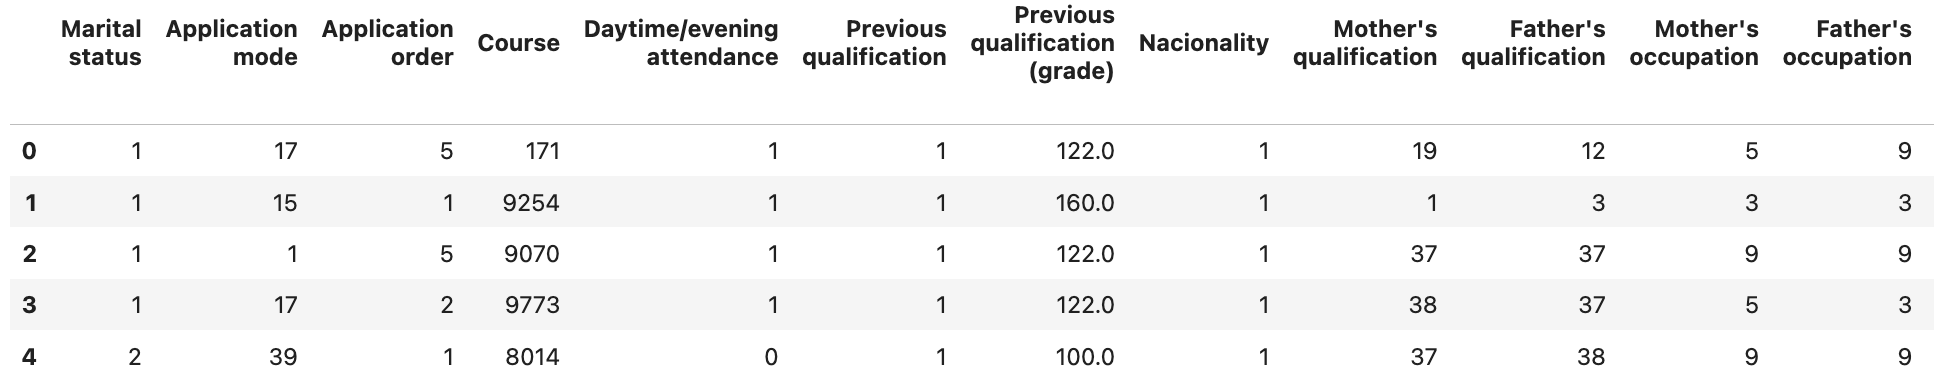
\includegraphics[width=0.9\textwidth]{./raw-data1.png}
    \caption{Snippet of the raw dataset (part 1).}
    \label{fig:raw1}
\end{figure}

\begin{figure}[H]
    \centering
    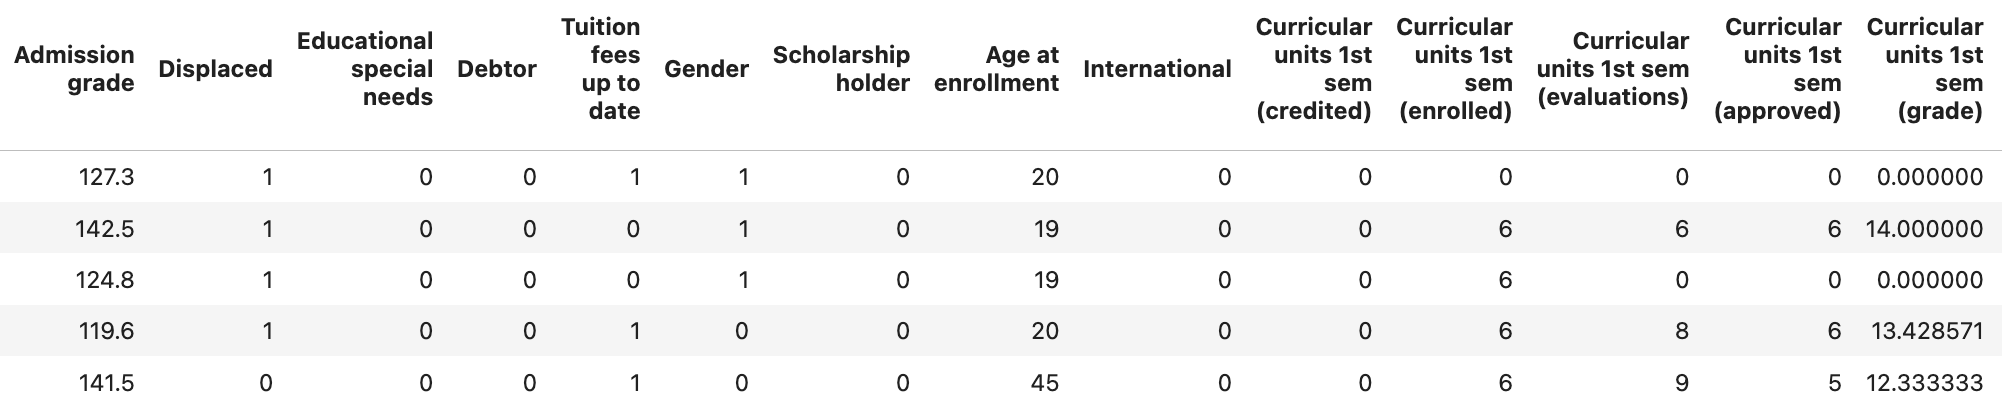
\includegraphics[width=0.9\textwidth]{./raw-data2.png}
    \caption{Snippet of the raw dataset (part 2).}
    \label{fig:raw2}
\end{figure}

\begin{figure}[H]
    \centering
    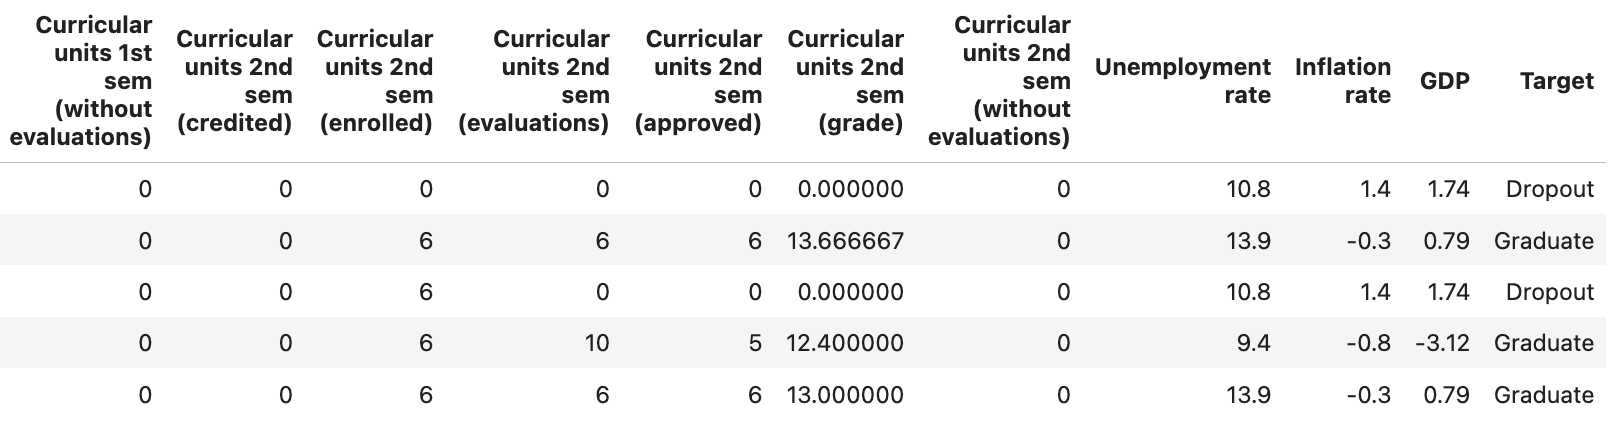
\includegraphics[width=0.9\textwidth]{./raw-data3.png}
    \caption{Snippet of the raw dataset (part 3).}
    \label{fig:raw3}
\end{figure}

To begin describing the implementation in concrete terms, we analyzed the dataset and identified that \textbf{18 out of the original 36 features were categorical or nominal}. They were:

\begin{itemize}
    \item Marital status
    \item Application mode
    \item Application order
    \item Course
    \item Daytime/evening attendance
    \item Previous qualification
    \item Nacionality
    \item Mother's qualification
    \item Father's qualification
    \item Mother's occupation
    \item Father's occupation
    \item Displaced
    \item Educational special needs
    \item Debtor
    \item Tuition fees up to date
    \item Gender
    \item Scholarship holder
    \item International
\end{itemize}

These features were therefore removed.

Next, we examined the distribution of dropout versus non-dropout labels to verify that the labels had a reasonably balanced distribution. We found that approximately \textbf{67.88\%} of students were classified as non-dropouts (either enrolled or graduated), while \textbf{32.12\%} were labeled as dropouts. This level of class imbalance was considered acceptable for proceeding with model training without requiring additional rebalancing techniques.

Thus, we transformed the target labels for binary classification by assigning a value of \texttt{1} to students labeled as \textit{Enrolled} or \textit{Graduate} and a value of \texttt{-1} to those labeled as \textit{Dropout}.

Next, we statistically analyzed the instances across each remaining (ordinal) feature to determine the most appropriate scaling technique. Specifically, we examined the \textbf{maximum}, \textbf{minimum}, \textbf{mean}, and \textbf{median} values to assess the distribution of values and detect potential outliers. Below are our notable findings:

\begin{enumerate}
    \item \textbf{Age at Enrollment}:
    \begin{itemize}
        \item Maximum: 70.00
        \item Mean: 23.27
        \item Median: 20.00
    \end{itemize}
    The maximum age is significantly higher than both the mean and median, indicating a strong right-skew and the presence of high-value outliers.

    \item \textbf{Curricular Units 1st Semester (Evaluations)}:
    \begin{itemize}
        \item Maximum: 45.00
        \item Mean: 8.30
        \item Median: 8.00
    \end{itemize}

    \item \textbf{Curricular Units 2nd Semester (Evaluations)}:
    \begin{itemize}
        \item Maximum: 33.00
        \item Mean: 8.06
        \item Median: 8.00
    \end{itemize}
    In both semesters, the maximum number of evaluations is considerably higher than the mean.

    \item \textbf{Inflation Rate}:
    \begin{itemize}
        \item Maximum: 3.70
        \item Mean: 1.23
        \item Median: 1.40
    \end{itemize}
    The inflation rate has a somewhat elevated maximum relative to the mean and median, but the variation is modest.

    \item \textbf{GDP}:
    \begin{itemize}
        \item Minimum: -4.06
        \item Mean: 0.002
        \item Median: 0.32
    \end{itemize}
    The minimum GDP value is notably lower than the average range, indicating a potential low-end outlier.
\end{enumerate}

While these features contain outliers, we chose not to remove them, as they appear to be \textit{contextually valid} within the domain of the dataset. 

Given that the ordinal features in our dataset generally have known and bounded domains, we decided to apply the \texttt{MinMaxScaler} from the \texttt{scikit-learn} package. This transformation rescales each feature individually to the range \([0,1]\) based on the formula:

\[
x' = \frac{x - x_{\text{min}}}{x_{\text{max}} - x_{\text{min}}}\, .
\]

As a result, the dataset was fully transformed and normalized to the \([0,1]\) range. The output of this preprocessing step is shown in the screenshots below:

\begin{figure}[H]
    \centering
    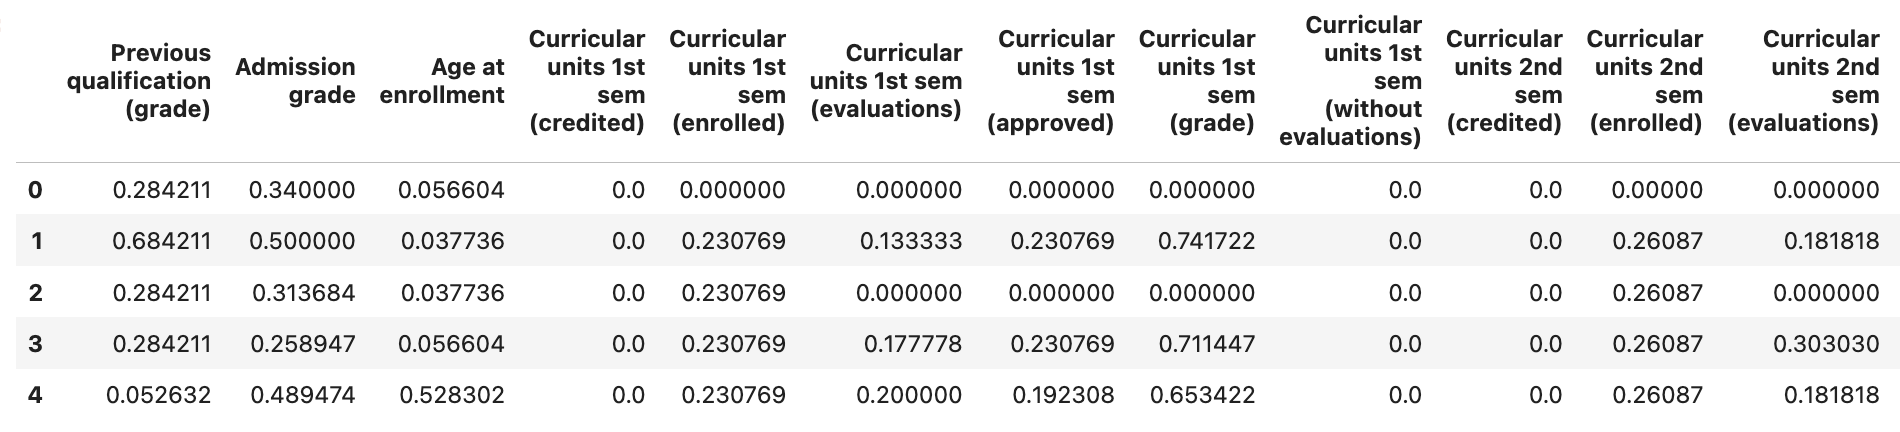
\includegraphics[width=0.9\textwidth]{./processed-data1.png}
    \caption{Scaled dataset after preprocessing (part 1).}
    \label{fig:proc1}
\end{figure}

\begin{figure}[H]
    \centering
    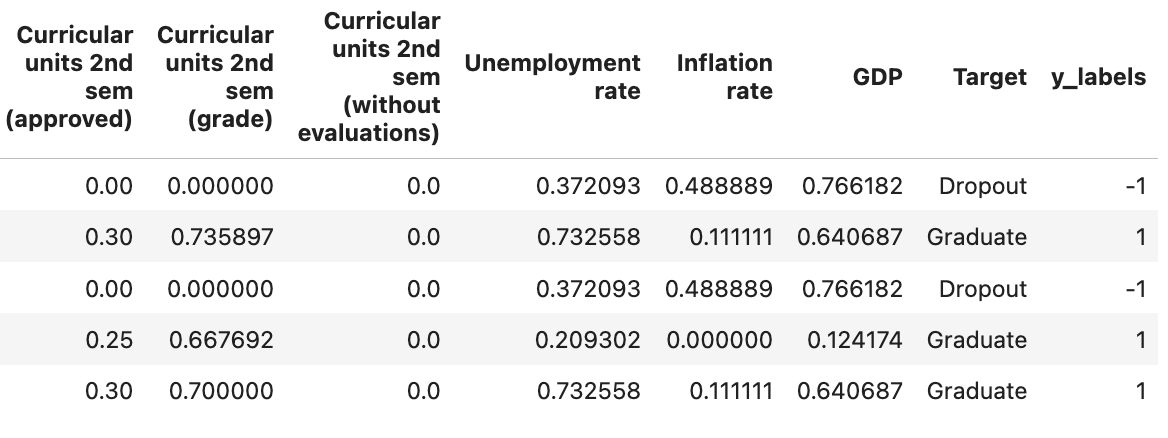
\includegraphics[width=0.9\textwidth]{./processed-data2.png}
    \caption{Scaled dataset after preprocessing (part 2).}
    \label{fig:proc2}
\end{figure}

%---------------------------------------------------
\section{Linear SVM using Stochastic Gradient Descent}

\subsection{Model Overview}

We implemented a \textbf{soft-margin linear SVM} with \textit{stochastic gradient descent} (SGD).  
For a training set $\{(x_i,y_i)\}_{i=1}^{n}$ with labels $y_i\in\{-1,+1\}$, the hinge-loss optimization problem is

\[
\min_{w,b}\;
\frac{1}{2}\lVert w\rVert^{2}
\;+\;
C\sum_{i=1}^{n}
\max\bigl(0,\,1 - y_i(w \cdot x_i + b)\bigr),
\]

where $C>0$ controls the trade-off between margin size and hinge-loss violations (i.e.\ slack variables).  
Because hinge loss and the $\ell_2$ penalty are both convex, the SGD procedure will converge to a minimizer under a diminishing step size.

\subsection{Training and Testing the Model}

\begin{enumerate}[label=\alph*)]
    \item \textbf{Data split}: The processed dataset was divided into 80\% training and 20\% testing.
    \item \textbf{Intercept term}: A column of ones was appended to $x$ so that the intercept $b$ is learned as an additional weight.
    \item \textbf{Update rule}: At each iteration $t$, we sampled one instance $(x_i,y_i)$ and updated the running parameter  
        \[
            \theta \leftarrow
            \begin{cases}
                \theta + y_i\,x_i &\text{if } y_i(w \cdot x_i)<1,\\[4pt]
                \theta &\text{otherwise},
            \end{cases}
        \]
        where $w_t=\dfrac{\theta}{2Ct}$.  
        The final weight vector is the time-average $\displaystyle w=\frac{1}{T}\sum_{t=1}^{T}w_t$.
    \item Regularization Term $C = 0.01$.
    \item $T=1{,}000$ iterations were (randomly) used to converge on the 3.5k training points.
\end{enumerate}

\begin{figure}[H]
    \centering
    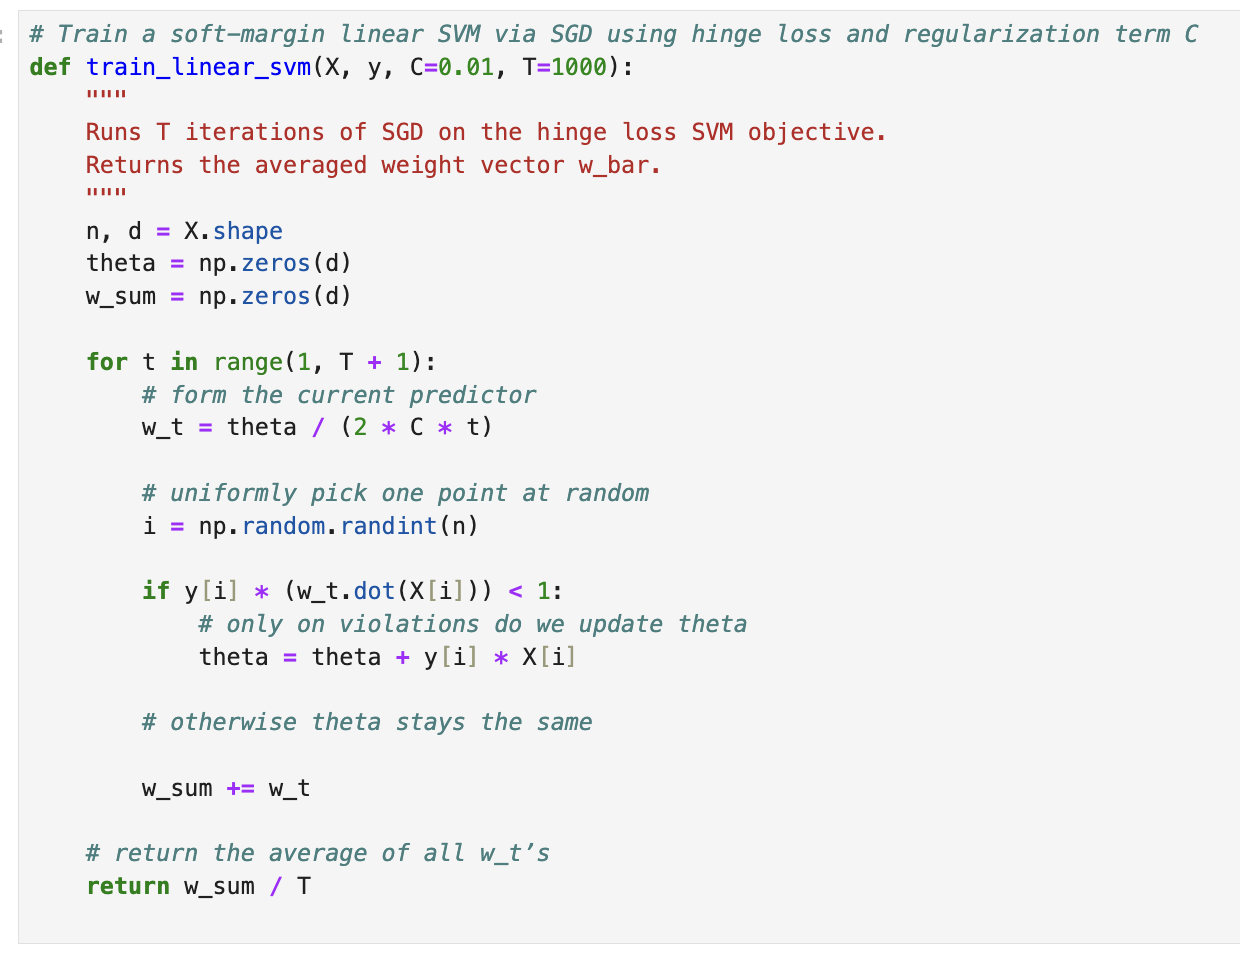
\includegraphics[width=0.92\textwidth]{./linear-svm-training-procedure.png}
    \caption{Python implementation of the SGD-based linear SVM.}
    \label{fig:sgd}
\end{figure}

The trained linear SVM produced the following coefficients and intercept:

\begin{table}[H]
\centering
\begin{tabular}{@{}l r@{}}
\toprule
\textbf{Feature} & \textbf{Coefficient} \\
\midrule
Intercept                                 & $-0.5773$ \\
Previous qualification (grade)            & $-0.0590$ \\
Admission grade                           & $-0.0077$ \\
Age at enrollment                         & $-0.5452$ \\
Curricular units 1st sem (credited)       & $-0.0174$ \\
Curricular units 1st sem (enrolled)       & $-0.2587$ \\
Curricular units 1st sem (evaluations)    & $-0.2724$ \\
Curricular units 1st sem (approved)       & $ 0.5804$ \\
Curricular units 1st sem (grade)          & $ 0.8073$ \\
Curricular units 1st sem (without eval.)  & $-0.0482$ \\
Curricular units 2nd sem (credited)       & $ 0.0207$ \\
Curricular units 2nd sem (enrolled)       & $-0.3253$ \\
Curricular units 2nd sem (evaluations)    & $-0.0777$ \\
Curricular units 2nd sem (approved)       & $ 1.0302$ \\
Curricular units 2nd sem (grade)          & $ 1.9480$ \\
Curricular units 2nd sem (without eval.)  & $-0.1016$ \\
Unemployment rate                         & $-0.0159$ \\
Inflation rate                            & $ 0.0068$ \\
GDP                                       & $-0.0267$ \\
\bottomrule
\end{tabular}
\caption{Learned feature coefficients from the trained linear SVM.}
\label{tab:coeffs}
\end{table}

Using the learned coefficients and intercept, the model achieved an accuracy of \textbf{82.0\%} on the test dataset.

\subsection{Identifying Significant Features via 5-Fold Cross-Validation}

While a soft-margin linear SVM addresses non-linearly separable data, it is inherently limited to finding a linear decision boundary in the original feature space. Given the structure of our dataset—comprising complex, interrelated academic and demographic factors—it is reasonable to assume that the true boundary between dropout and non-dropout cases is non-linear.

To address this, we turn to a very powerful class of models: \textbf{kernel-based SVMs} trained using \textbf{dual optimization}. These models operate by implicitly mapping the original feature vectors into a higher-dimensional space via a kernel function (e.g., polynomial or Gaussian), where linear separation is more likely to be achievable.

This approach allows the SVM to model more complex relationships between features without explicitly computing the high-dimensional transformation, thanks to the kernel trick. 

Nevertheless, to maximize our use of the linear SVM, we leveraged it as a tool for \textbf{statistical feature analysis}. We can analyze the learned coefficients to identify the most significant features that contribute to the classification performance.

To do this, we employed a \textbf{five-fold cross-validation} procedure using \texttt{KFold} from the \texttt{scikit-learn} library. We explicitly set \texttt{shuffle=False} to ensure that the fold partitions remained fixed across runs. This helped maintain consistency in how each feature contributed to the model.

Cross-validation was conducted on the 80\% training set, with each fold splitting the data into 60\% for training and 20\% for validation. In each fold, the linear SVM was trained on the 60\% subset and evaluated on the corresponding 20\% validation set. We recorded both the learned weight vector and validation accuracy in each iteration. The average cross-validation performance was:

\[
\text{CV accuracy} = 0.805 \pm 0.004\, .
\]

We evaluated several statistical metrics from the cross-validation, which produced the following results:

\begin{figure}[H]
    \centering
    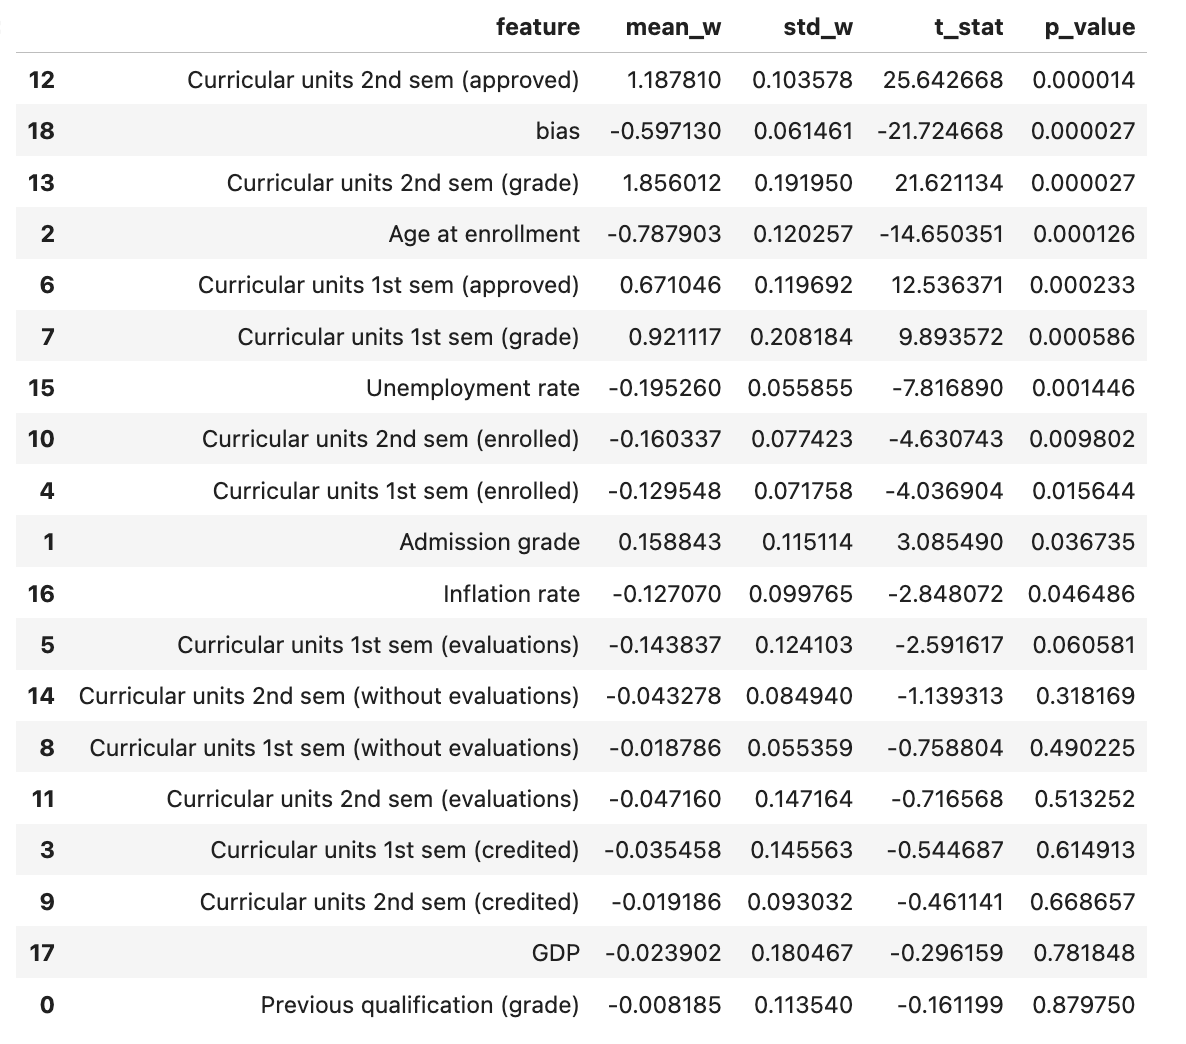
\includegraphics[width=0.9\textwidth]{./statistical-analysis-of-ordinal-features.png}
    \caption{Statistical analysis of feature weights across fixed five-fold cross-validation.}
    \label{fig:stats}
\end{figure}

Based on these, features with a $p$-value less than 0.05 were considered \textbf{statistically significant} and retained for further modeling. Conversely, features with $p$-values greater than or equal to 0.05 were excluded from the dataset.

\textbf{Significant Features} ($p < 0.05$):
\begin{itemize}
  \item Curricular units 2nd sem (approved)
    \item Curricular units 2nd sem (grade)
    \item Age at enrollment
    \item Curricular units 1st sem (approved)
    \item Curricular units 1st sem (grade)
    \item Unemployment rate
    \item Curricular units 2nd sem (enrolled)
    \item Curricular units 1st sem (enrolled)
    \item Admission grade
    \item Inflation rate
\end{itemize}

\textbf{Non-Significant Features} ($p \ge 0.05$):
\begin{itemize}
    \item Curricular units 1st sem (evaluations)
    \item Curricular units 2nd sem (without evaluations)
    \item Curricular units 1st sem (without evaluations)
    \item Curricular units 2nd sem (evaluations)
    \item Curricular units 1st sem (credited)
    \item Curricular units 2nd sem (credited)
    \item GDP
    \item Previous qualification (grade)
\end{itemize}

The non-significant features were removed from the dataset, resulting in a refined feature set. The following represents the updated dataset to be used for our kernel-based SVM model:

\begin{figure}[H]
    \centering
    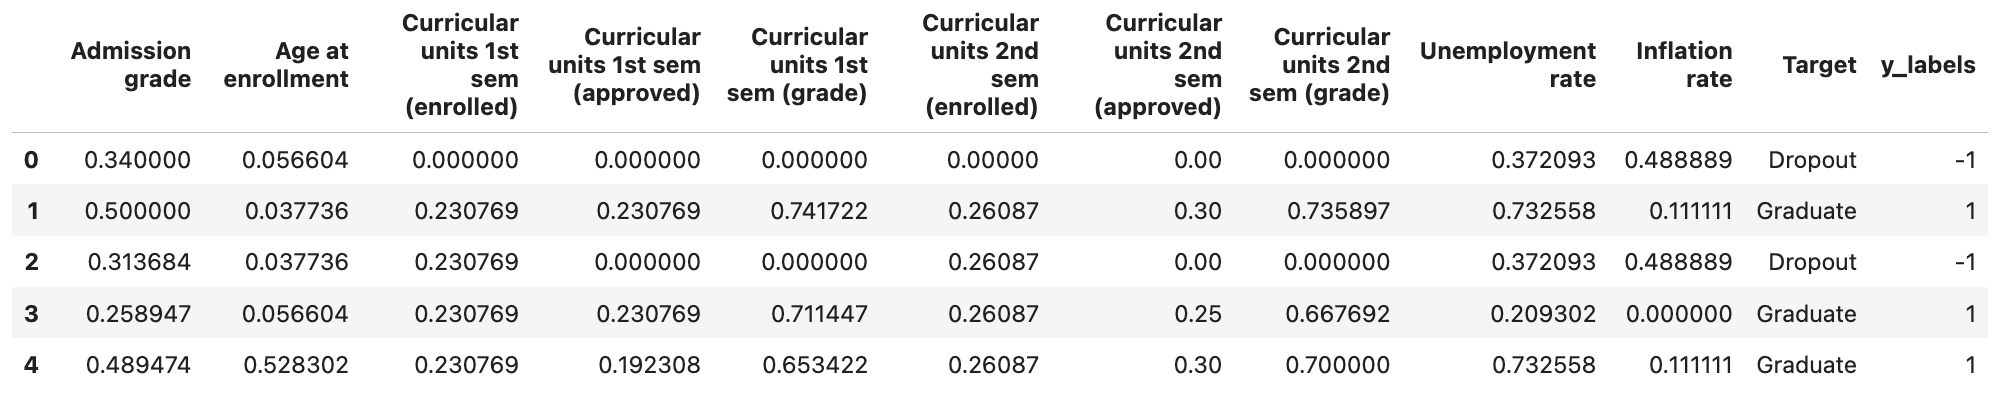
\includegraphics[width=0.9\textwidth]{./significant-features-dataset.png}
    \caption{Updated dataset containing only the most significant features.}
    \label{fig:sigdata}
\end{figure}

%---------------------------------------------------

\section{Kernel-based Support Vector Machine} 

\subsection{Model Description and Rationale}

To capture non-linear relationships that a soft-margin linear SVM cannot model, we solve the dual optimization problem:

\[
\begin{aligned}
\max_{\boldsymbol{\alpha}}\quad
&\sum_{i=1}^n \alpha_i
 \;-\;
 \frac{1}{2}\sum_{i=1}^n\sum_{j=1}^n 
 \alpha_i\,\alpha_j\,y_i\,y_j\,(x_i \cdot x_j)
 \\[4pt]
\text{subject to}\quad
&\alpha_i \ge 0 \quad (i=1,\dots,n),\\[4pt]
&\sum_{i=1}^n \alpha_i\,y_i = 0.
\end{aligned}
\]

Because this formulation depends only on the inner product \(x_i\cdot x_j\), we can replace it with a kernel function \(K(x_i,x_j)\). In our experiments, we use both the polynomial and Gaussian kernels. The regularization constant \(C\) still governs the trade-off between margin width and hinge-loss violations, and the dual variables \(\alpha_i\) are found via stochastic gradient descent. This “kernel trick” lets us learn a non-linear decision boundary in the original feature space without ever explicitly computing a high-dimensional feature map.  

We considered two kernels:

\begin{itemize}
  \item \textbf{Polynomial Kernel}\,: $K_{\text{poly}}\!(x,x') = (\gamma\,(x{\cdot}x') + r)^{d}$
  \item \textbf{Gaussian Kernel}\,: $K_{\text{rbf}}\!(x,x') = \exp[-\gamma \lVert x - x'\rVert^{2}]$
\end{itemize}

\subsection{Training Procedure}
The dataset containing only statistically significant features was split into \textbf{80\,\% training} and \textbf{20\,\% test} sets using \texttt{train\_test\_split} from \texttt{scikit-learn}.

\vspace{0.5ex}
We implemented the training procedure for the kernel SVM using \textbf{stochastic gradient descent}. This method updates the dual variables $\alpha_i$ iteratively based on hinge-loss violations:

\begin{itemize}
  \item At each iteration $t$, randomly select a data point $(x_j, y_j)$,
  \item Compute the margin violation using the precomputed kernel Gram matrix,
  \item If the point violates the margin (i.e.\ $ y_j f(x_j) < 1 $), set $\beta_j \leftarrow \beta_j + y_j$,
  \item Compute $\alpha^{(t)} = \beta / (2 C t)$ and average across $T = 1000$ iterations to obtain the final dual solution $\bar{\alpha}$.
\end{itemize}

\begin{figure}[H]
    \centering
    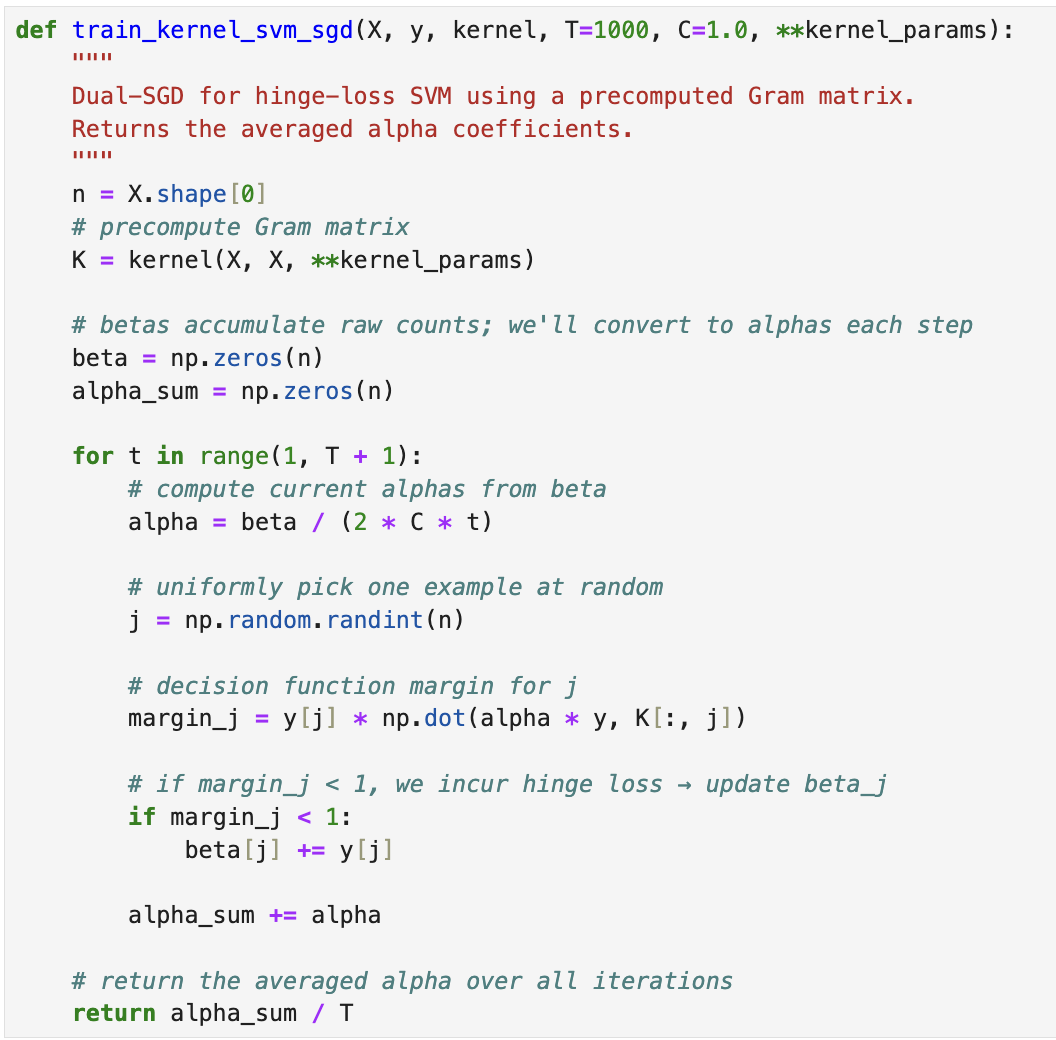
\includegraphics[width=0.9\textwidth]{./kernel-svm-training-procedure.png}
    \caption{Implementation of the training procedure for dual-SGD SVM.}
    \label{fig:kertrain}
\end{figure}

\subsection{Tuning Hyperparameters}

We conducted a \textbf{grid search} with five-fold cross validation over combinations of kernel hyperparameters—specifically, the polynomial degree $d$, kernel coefficient $\gamma$, offset $r$, and regularization constant $C$—using \texttt{ParameterGrid} from \texttt{scikit-learn}.  

\begin{table}[H]
\centering
\begin{tabular}{@{}ll@{}}
\toprule
\textbf{Kernel} & \textbf{Grid} \\ \midrule
Polynomial & $d \in \{2, 3, 4\}$,\; $\gamma \in \{10^{-4},\dots,1\}$,\; $r \in \{0, 0.5, 1, 2\}$,\; $C \in \{10^{-4},\dots,10\}$ \\
Gaussian   & $\gamma \in \{10^{-5},\dots,3\}$,\; $C \in \{10^{-4},\dots,10\}$ \\ 
\bottomrule
\end{tabular}
\caption{Hyperparameter grid used for polynomial and RBF kernel SVMs.}
\label{tab:grid}
\end{table}

This procedure yielded the following optimal configurations:

\begin{itemize}
    \item \textbf{Polynomial kernel:}\\
    Best parameters \{C = 0.001, degree = 3, $\gamma$ = 0.1, $r$ = 0\},\\
    \item \textbf{Gaussian kernel:}\\
    Best parameters \{C = 0.1, $\gamma$ = 3\},\\
\end{itemize}

\subsection{Model Training and Testing Evaluation}

We then refitted the full training set with the optimal parameters (Polynomial: \{$d=3,\gamma=0.01,r=1,C=0.3$\}; Gaussian: \{$\gamma=0.03,C=3$\}).

The test-set performance of our two kernel SVM models is summarized in Table~\ref{tab:test_metrics}. Four standard metrics are reported:

\begin{itemize}
  \item \textbf{Accuracy}: fraction of all students whose outcome (dropout vs.\ non-dropout) was predicted correctly.
  \item \textbf{Log-Loss}: negative log-likelihood of the true labels under the model’s predicted probabilities (lower is better).
  \item \textbf{Precision}: among students predicted to drop out, the fraction who actually did.
  \item \textbf{Recall}: among students who truly dropped out, the fraction correctly identified.
\end{itemize}

\begin{table}[H]
\centering
\begin{tabular}{lcccc}
\toprule
\textbf{Kernel} & \textbf{Accuracy} & \textbf{Log-Loss} & \textbf{Precision} & \textbf{Recall} \\ \midrule
Polynomial & $0.8147$ & $6.6793$ & $0.8073$ & $0.9551$ \\
Gaussian   & $0.8215$ & $6.4349$ & $0.8160$ & $0.9517$ \\ 
\bottomrule
\end{tabular}
\caption{Test-set metrics for the best polynomial and Gaussian kernel SVMs.}
\label{tab:test_metrics}
\end{table}

\subsection{Ablation Check: Re-adding Dropped Ordinal Features}

\paragraph{Purpose.}
We sought to verify that the earlier feature-selection step did not strip away any useful contributions to the classification prediction and so we refitted both kernel SVMs on the \emph{entire} ordinal feature matrix. The hyperparameter grid search was repeated on this superset after which the models were re-fit and evaluated on the procedure.

\begin{table}[H]
\centering
\begin{tabular}{lccccc}
\toprule
Kernel & Accuracy & Log-Loss & Precision & Recall\\ \midrule
Polynomial (all) & $0.8158$ & $6.6385$ & $0.8102$ & $0.9517$ \\
Gaussian (all)   & $0.8158$ & $6.6385$ & $0.8085$ & $0.9551$ \\ 
\bottomrule
\end{tabular}
\caption{Performance after re-introducing all ordinal features.}
\label{tab:full_feats}
\end{table}

\paragraph{Take-away.}
The performance is virtually identical to that in Table~\ref{tab:test_metrics}, confirming that the non-significant features did not contribute much to the classification problem. Retaining only the statistically significant features thus simplifies the model without sacrificing performance.

\subsection{Final Results and Summary}

\paragraph{Kernel-based SVM Interpretation.}  
Both kernel SVM models demonstrate a solid predictive performance on the student dropout task, with the Gaussian kernel slightly outperforming the polynomial kernel overall. The polynomial SVM achieves 81.47\% accuracy, 0.8073 precision, and 0.9551 recall, while the Gaussian SVM reaches 82.15\% accuracy, 0.8160 precision, and 0.9517 recall. Both models maintain high recall—above 95\%—indicating they successfully identify nearly all true dropouts, and their precision values around 80\% show a reasonable balance between avoiding false alarms and catching at-risk students. Overall, these results suggest that kernelized SVMs can reliably flag students at risk of dropping out, with the Gaussian kernel offering a slight edge.

\paragraph{Comparison to linear model.}  
Interestingly, the Gaussian kernel’s 82.15\% accuracy matches our soft-margin linear SVM baseline (82.0\%), while the polynomial kernel is slightly below. This suggests that the relationship between the selected features and dropout risk is largely linear--contrary to our initial assumption--and that mapping into a higher-dimensional feature space yields only marginal gains.

\paragraph{Challenges and limitations.}
\begin{itemize}
  \item \textbf{Computational cost}: Each full grid search (polynomial plus Gaussian) required approximately 10-15 minutes of CPU time, limiting the size of the hyperparameter grids we could explore (which could greatly explain why we're not seeing larger improvements over the linear SVM).
    \item \textbf{Feature scope}. The ablation study proves that reintroducing the statistically insignificant ordinal features does not improve performance. However, the apparent linearity of the data possibly suggests that removing the categorical and nominal variables may have removed useful information. Future work should either develop effective encodings for those features (despite the challenges encoding has for distance-based algorithms) or to actually explore other models besides SVMs.
\end{itemize}

\paragraph{Key takeaways.}
\begin{itemize}
  \item The Gaussian kernel SVM achieved 82.15\% accuracy and 0.8160 precision—0.68 pp higher precision than the polynomial kernel—demonstrating a modest gain from non-linear mapping.
  \item The linear SVM baseline matched kernel performance (82.10\% vs.\ 82.15\%), indicating that our 10 statistically significant ordinal features capture the bulk of the predictive signal.
  \item Reintroducing the 8 non-significant ordinal features (e.g.\ GDP, previous qualification, credited units) did not alter accuracy (0.8158\%), confirming that the refined 10-feature set suffices.
  \item Semester grades dominate feature importance: “Curricular units 2nd sem (grade)” has the largest coefficient (1.9480), followed by “Curricular units 1st sem (grade)” (0.8073), whereas economic factors like inflation (0.0068) and GDP (–0.0267) contribute minimally.
  \item All SVM variants maintain recall above 95\%, effectively flagging at-risk students, though false-positive rates of ~15–17\% suggest potential value in cost-sensitive threshold tuning.
\end{itemize}


\end{document}